\section{Scope of the Thesis}

The present-day noisy intermediate-scale quantum computers are capable of running simple quantum procedures, and in the case of some special problems, they come close to showing a significant quantum advantage over their classical counterparts \cite{google-quantum-supremacy}. However, we are still a long way off from the goal of performing general-purpose computation to solve meaningful problems with a significant speedup over the classical realm. The path to making quantum computation feasible will involve iterated progress in several domains, like the following. 
\begin{enumerate}
    \item Building hardware with a larger number of qubits which have better noise-resilliance and higher connectivity for multi-qubit operations across those qubits. 
    \item Designing quantum error detection codes to mitigate noise by composing a single logical qubit from many physical qubits.
    \item \label{item:thesis-motivations-algorithms} Coming up with quantum algorithms to solve problems of practical value which are intractable on classical computers.
    \item \label{item:thesis-motivations-compiling} Compiling those algorithms down to circuit operations such that they can be carried out quickly and reliably.
\end{enumerate}

This focus of the work in this dissertation is to address points \ref{item:thesis-motivations-algorithms} and \ref{item:thesis-motivations-compiling}.

\subsection{Research Problems tackled}

\begin{enumerate}\label{enum:problems-addressed-by-thesis}
    \item[\textbf{T1}] \textit{To incorporate the notion of parallelizability and noise mitigation in Quantum Circuits in Machine Learning based circuit routing algorithms}
    The longer quantum circuits take to execute, the more noise and decoherence of the quantum state affect the final results. Quantum states decohere even quicker when no operations are being applied to them, which is when they are waiting for parts of the circuit to finish. Planning methods to execute circuits with the least number of gates do exist, but we need to add the notion of parallel operations into this planning process, as well as in any neural process that helps guide it.

    \item[\textbf{T2}] \textit{To design an algorithm for efficient and neurally-guided search in combinatorially large search spaces.}
    A parallelizable set of actions need to be scheduled at each time-step by our planner. The number of possible sets of operations we are deciding over is exponential in the size of the hardware. Since searching over all sets is infeasible, all methods to iteratively add or remove elements from the set in order to come up with some heuristic maximization. We attempt to come up with one such method which would allow us to stably train our networks in this RL setting.

    \item[\textbf{T3}] \textit{To develop a framework for analyzing variational algorithms on noisy-quantum computers, evaluating the quantum advantage, convergence properties of the learning process, etc.}
    Variational Methods \ref{sec:variational-circuits} are typically used to solve hard optimization problems, in which the classical sub-system learns parameters for a Parametrized Quantum Circuit (PQC) to maximize some function of the state prepared by said circuit. This is, in essence, a learning algorithm, and analysis of these learning algorithms and iterating on designs of these circuits should be both based on intuition from other quantum algorithms (in the way QAOA is inspired from quantum annealing and trotterization \ref{sec:variational-circuits-qaoa}) and from data obtained about the loss landscape on which we are optimizing.
\end{enumerate}

\section{Motivation}

\subsection{qRoute: Qubit Routing}

\begin{figure}[H]
    \centering
    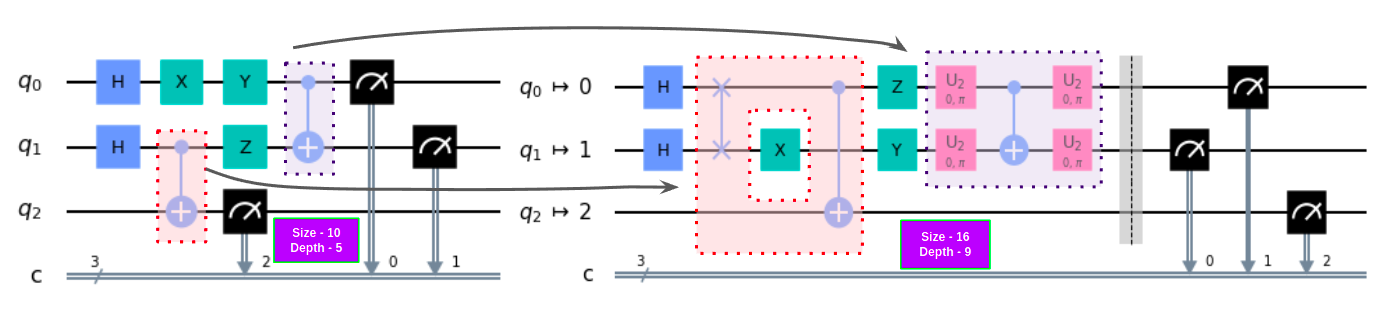
\includegraphics[width=\linewidth]{figures/intro/routing-transform.png}
    \caption{Transformation of a Quantum Circuit where non-local operations are scheduled to one implementable on the hardware (qubits 1 and 2 are not a local pair, 0 and 1, and 0 and 2 are). The decomposition of some gates is shown with arrows.}
\end{figure}

The value of the entire set of actions is largely dependent on the independent value of actions in the set, and the values added by the co-occurrance of small subsets of these actions, i.e. operations occuring on qubits significantly separated on hardware do not affect each other. This 

\subsection{qLEET: Variational Circuit Visualization}

\begin{figure}[H]
    \centering
    \hfill
    \begin{subfigure}[b]{0.45\linewidth}
        \centering
        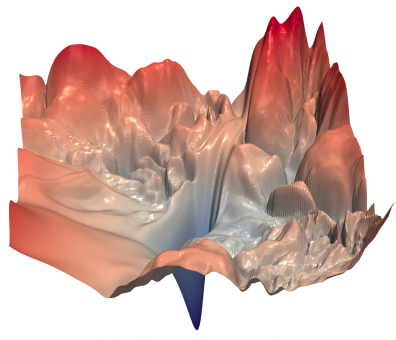
\includegraphics[width=0.7\textwidth]{figures/intro/landscape-rough.png}
        \caption{Loss Landscape without Skip Connections\label{fig:loss-landscape-rough}}
    \end{subfigure}
    \hfill
    \begin{subfigure}[b]{0.45\linewidth}
        \centering
        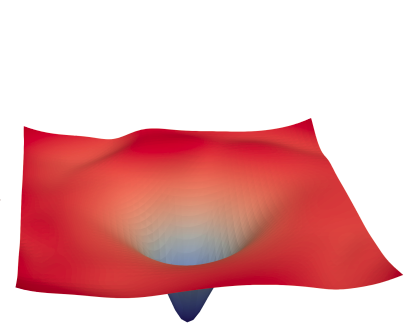
\includegraphics[width=0.7\textwidth]{figures/intro/landscape-smooth.png}
        \caption{Loss Landscape with Skip Connections\label{fig:loss-landscape-smooth}}
    \end{subfigure}
    \hfill
    \caption{The loss landscapes of neural networks with and without skip connections, as visualized by Li et. al.\cite{loss-landscapes}. The architectural decision of adding skip connections makes the feasibility of the optimization process a lot higher, to the extent visualizable on a 2-D random projection.}
    \label{fig:loss-landscape-neural-nets}
\end{figure}

\section{Thesis Layout}

\begin{itemize}
    \item[C1] This is the introductory chapter, which discusses the scope of the work carried out in this thesis in the context of developments in quantum computation, addresses the problems we are attempting to pose solutions to, and adds some motivation for the methods that we will develop in the following chapters.
    \item[C2] Here we presents a background in Quantum Computing and Reinforcement Learning which is requisite for understanding the motivations of the methods developed and the algorithms used in the remainder of this dissertation. We conclude this chapter by enlisting some ideas that we are going to use to address the problems posed in \ref{enum:problems-addressed-by-thesis}.
    \item[C3] As the first major contribution of this thesis, we present \textbf{qRoute: Qubit Routing using Graph Neural Network aided Monte Carlo Tree Search}, which is a reinforcement learning algorithm we propose for depth-minimized (used as a proxy for noise-mitigated) compilation. We discuss the problem of routing problem, discuss the specifics of our algorithm and associated neural architecture design.
    \item[C4] The other contribution of this thesis is \textbf{qLEET: Visualizing Loss Landscapes, Expressibility, Entangling power and Training Trajectories for Parameterized Quantum Circuits}, in which we present a way to analyze the properties of variational methods that can be implemented on present day quantum computers, and build a software framework for the same.
    \item[C5] We conclude with a summary of methods and results discussed in this thesis and the scope of extension of this work in the future.
\end{itemize}

